\documentclass{standalone}
\usepackage{tikz}
\usepackage{ctex,siunitx}
\usepackage{tkz-euclide}
\usepackage{amsmath}
\usetikzlibrary{patterns, calc}
\usetikzlibrary {decorations.pathmorphing, decorations.pathreplacing, decorations.shapes,}
\begin{document}
\small
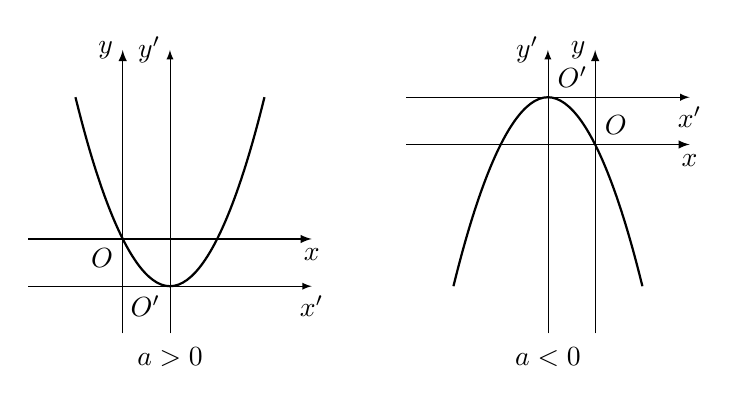
\begin{tikzpicture}[>=latex,scale=0.6]
  \begin{scope}
    \draw[very thin,->](-2,-1)--(4,-1)node[below]{$x'$};
    \draw[very thin,->](1,-2)--(1,4)node[left]{$y'$};
    \draw[thin,->](-2,0)--(4,0)node[below]{$x$};
    \draw[thin,->](0,-2)--(0,4)node[left]{$y$};
    \node at (0,0)[below left]{$O$};
    \node at (1,-1)[below left]{$O'$};
    \draw[thick](-1,3) parabola bend (1,-1) (3,3);
    \node at (1,-2.5){$a>0$};
  \end{scope}
  \begin{scope}[xshift=10cm,yshift=2cm]
    \draw[very thin,->](-4,1)--(2,1)node[below]{$x'$};
    \draw[very thin,->](-1,-4)--(-1,2)node[left]{$y'$};
    \draw[thin,->](-4,0)--(2,0)node[below]{$x$};
    \draw[thin,->](0,-4)--(0,2)node[left]{$y$};
    \node at (0,0)[above right]{$O$};
    \node at (-1,1)[above right]{$O'$};
    \draw[thick](-3,-3) parabola bend (-1,1) (1,-3);
    \node at (-1,-4.5){$a<0$};
  \end{scope}
\end{tikzpicture}
\end{document}